\chapter{Empirical Validation}
\label{chap:empirical-validation}

When a new programming model is proposed, it must be demonstrated that
interesting programs can be written within the model.  While the model
espoused by this thesis---functional array programming---is not new,
our claim that it is a good foundation for obtaining parallel
performance requires evidence.

This chapter serves as an empirical validation of the compilation
strategy discussed in this thesis, and the practical usability of the
Futhark compiler as a whole (the \textit{fifth contribution} from the
introduction).  We discuss several programs implemented in Futhark,
with a focus on their runtime performance.  While we cannot claim that
the current Futhark compiler embodies the full potential of functional
array programming, the results presented here constitute at least a
lower bound on that potential.

The chapter is divided into two main parts: first we have manually
translated a range of benchmark programs from other languages or
libraries to Futhark (\cref{sec:bulk-benchmarking}).  Second, we
perform a deeper analysis of the performance of an irregular program
that, due to dataset-sensitivity, is not as easy to benchmark
(\cref{sec:bfs-benchmarking}).  We will use the term \textit{reference
  implementation} to refer to programs that were not written by us,
and \textit{Futhark implementation} to refer to our translated Futhark
programs.  Any Futhark code examples will use the source language, not
the IR we used to discuss the design of the compiler.

\section{Empirical Validation in Bulk}
\label{sec:bulk-benchmarking}

\newcommand\results[1]{\input{img/runtimes/#1-ref.tex} & \input{img/runtimes/#1-futhark.tex} & \input{img/runtimes/#1-auxref.tex} & \input{img/runtimes/#1-auxfuthark.tex} }

\begin{table}
  \centering
  \begin{tabular}{ll||rr|rr}
    & & \multicolumn{4}{c}{\textbf{Runtime in milliseconds}} \\
     & & \multicolumn{2}{c|}{\textbf{NVIDIA K40}} & \multicolumn{2}{c}{\textbf{AMD W8100}} \\
    \textbf{Benchmark} & \textbf{Dataset} & \textbf{Ref.} & \textbf{Fut.} & \textbf{Ref.} & \textbf{Fut.}  \\\hline
    \\\textbf{Rodinia} \\\hline
    Backprop & Input layer size equal to $2^{20}$ & \results{backprop} \\
    CFD & fvcorr.domn.193K & \results{cfd} \\
    HotSpot & $1024\times1024$; $360$ iterations & \results{hotspot} \\
    $k$-means & kdd\_cup & \results{kmeans} \\
    LavaMD & $\texttt{boxes1d}=10$ & \results{lavaMD} \\
    LUD & $2048$ & \results{lud} \\
    Myocyte & $\texttt{workload}=2^{16}$; $\texttt{xmax}=3$ & \results{myocyte} \\
    NN & Default duplicated $20$ times & \results{nn} \\
    Pathfinder & Array of size $10^{5}$ & \results{pathfinder} \\
    SRAD & $502\times458$; $100$ iterations & \results{srad} \\
    \\\textbf{Parboil} \\\hline
    MRI-Q & large & \results{mri-q} \\
    SGEMM & medium & \results{sgemm} \\
    Stencil & default & \results{stencil} \\
    TPACF & medium & \results{tpacf} \\
    \\\textbf{FinPar} \\\hline
    \multirow{3}{*}{LocVolCalib} & small & \results{LocVolCalib_small} \\
    & medium & \results{LocVolCalib_medium} \\
    & large & \results{LocVolCalib_large} \\
    \multirow{3}{*}{OptionPricing} & small & \results{OptionPricing_small} \\
    & medium & \results{OptionPricing_medium} \\
    & large & \results{OptionPricing_large} \\
    \\\textbf{Accelerate} \\\hline
    Crystal & Size $2000$, degree $50$ & \results{crystal} \\
    Fluid & $3000\times3000$; 20 iterations & \results{fluid} \\
    Mandelbrot & $4000\times4000$; 255 limit & \results{mandelbrot} \\
    N-body & $N=10^{5}$ & \results{nbody} \\
    Tunnel & $4000\times{}4000$ & \results{tunnel} \\
  \end{tabular}
  \caption{Benchmark datasets and average runtimes, computed over ten
    executions of every benchmark.  See
    \cref{fig:rodinia-speedup,fig:parboil-speedup,fig:finpar-speedup,fig:accelerate-speedup}
    for a visualisation of the results.  Missing entries indicate that
    a benchmark implementation was not runnable for a given
    configuration.}
  \label{tab:benchmarks}
\end{table}

Most of the programs presented in this section are from the published
benchmark suites Rodinia 3.1~\cite{5306797}, Parboil
2.5~\cite{stratton2012parboil}, and FinPar~\cite{FinPar:TACO}.  The
comparison with hand-written implementations is to show the potential
cost of using a high-level language.  However, as we shall see, even
published code often contains significant inefficiencies, which
occasionally leads to Futhark outperforming the reference
implementations.  A handful of benchmarks are from Accelerate
1.0~\cite{mcdonell2013optimising}, a Haskell eDSL for data-parallel
array programming.  These are included to show the performance of
Futhark compared to an existing mature GPU language.

All programs have been manually ported to Futhark, and compiled and
run with the default settings.  We show how the performance of the
Futhark code compares to the performance of the original reference
implementations.  In some cases, we also discuss the programming
techniques used to obtain efficient Futhark implementations.  For most
benchmarks, we use only a single dataset, as the relative performance
for these is not dataset-sensitive (except for pathological cases).

While some of the benchmarks are small, others are decidedly
nontrivial.  For example, Stencil from Parboil is implemented as $13$
non-blank non-comment lines of Futhark, while Myocyte from Rodinia
requires $883$.  The total number of non-blank non-comment lines in
the Futhark implementations is $2984$, with a median of of $98$.

We have evaluated the performance of the generated code on two
different test systems:

\begin{enumerate}
\item An NVIDIA K40 GPU installed in a server-grade system with an
  Intel Xeon E5-2560 CPU and 128GiB of RAM.
\item An AMD W8100 GPU installed in a desktop-class system with an
  Intel Core 2 Quad CPU and 4GiB of RAM.
\end{enumerate}

The intent is to show that the OpenCL code generated by the Futhark
compiler works on both NVIDIA and AMD GPUs.  However, note that the
two systems are very dissimilar---the AMD GPU is installed in a rather
old computer, and it is possible that the slow CPU and anaemic amount
of system memory may bottleneck the GPU\footnote{Unusually, the GPU
  actually has \textit{more} memory than the CPU; a reversal of the
  usual situation.}.  This may explain some of the unusual behaviour
we will see on the AMD GPU, particularly for reference
implementations.  In particular, three reference implementations from
Rodinia---Backprop, Hotspot, and Pathfinder---exhibit extreme and
inexplicable slowdown on the AMD GPU.  We consider these results
anomalous, and will discard from from further discussion (although
they are included in the graphs and tables).  Ideally, the NVIDIA and
AMD GPUs would be installed in systems that are otherwise similar, but
such were not available for the writing of this thesis.

CUDA, as an API proprietary to NVIDIA, can be executed only on the
NVIDIA K40 GPU.  Thus, when selecting reference implementations, we
have picked those written in OpenCL, to allow us to run the same code
on both platforms.  Reference implementations in OpenCL were not
available for all benchmarks; these will be discussed on a
case-by-case basis.  All Futhark implementations executed successfully
on both test systems.

We invoke the Futhark compiler with no benchmark-specific flags---no
tuning is done, and the exact same code is executed on both of our
test systems.  It is likely that approximately 10\% speedup could be
obtained by tweaking GPU group sizes.

The compiler inserts instrumentation that records total runtime minus
the time taken for (i) loading program input onto the GPU, (ii)
reading \textit{final} results back from the GPU, and (iii) OpenCL
context creation and kernel build time.  Excluding these overheads
emphasises the performance differences.  Any other host-device
communication/copying is measured.  When necessary, the reference
implementations have been modified to time similarly.  When in doubt,
we have erred in favour of the reference implementations.

The results are shown on \cref{tab:benchmarks}, and discussed in
greater detail below.  Most of our slowdown is related to generic
issues of unnecessary copying and missing micro-optimisation that are
common to compilers for high-level languages.
\Cref{sec:impact-of-optimisation} contains a brief discussion of how
the major optimisations performed by the Futhark compiler affect the
performance of the benchmarks.

Futhark implementations of all benchmarks discussed here, as well as
several more, are publicly available at the following URL:

\centerline{\url{https://github.com/diku-dk/futhark-benchmarks}}

\subsection{Ten Benchmarks from Rodinia}
\label{sec:rodinia}

\begin{figure*}
  \centering
  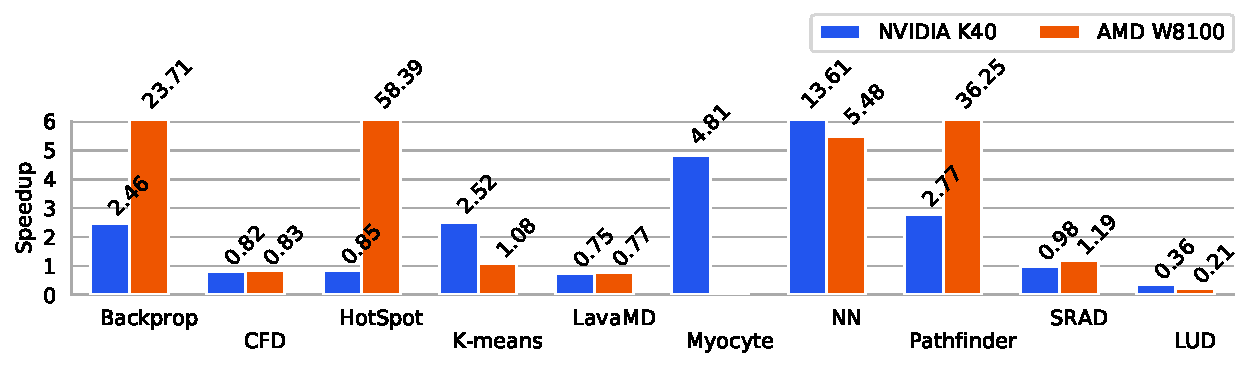
\includegraphics[scale=0.65]{experiments/rodinia.pdf}
  \caption{Relative speedup compared to reference implementations for
    Rodinia (the bar for NN is truncated for space reasons).}
  \label{fig:rodinia-speedup}
\end{figure*}

Rodinia is a popular benchmark suite that contains approximately $21$
benchmarks.  Of these, we have selected those $10$ benchmarks that
look the most friendly from a data-parallel perspective, and were
expressible in terms of a nested composition of \kw{map}, \kw{reduce},
\kw{scan}, \StreamRed{}, \StreamMap{}.

There is great variation in the performance of the Rodinia reference
implementations.  Some, such as Myocyte or NN, contain oversights that
negatively affect GPU performance.  Others, such as LUD or LavaMD, are
based on clever algorithms and carefully implemented.  Some Rodinia
implementations exhibit massive slowdown on the AMD GPU for reasons
that we cannot determine.  We conjecture that this is related to the
under-powered CPU on the machine hosting the AMD GPU, but this is only
a suspicion.  The speedups are shown on \cref{fig:rodinia-speedup}.

The speedup on Backprop seems related to a reduction that Rodinia has
left sequential.  Running time of the training phase is roughly equal
in Rodinia and Futhark ($\sim10~ms$).

Rodinia's implementation of HotSpot, a two-dimensional stencil code,
uses time tiling~\cite{HexaTiling}, which seems to pay off on the
NVIDIA GPU, but not on AMD.  On the NVIDIA GPU, the majority of
Futhark's slowdown is due to how memory management is done for the
arrays involved in the time series loop in the stencil.  At a high
level, the stencil is a sequential loop containing a nested \kw{map}
over the $m\times{}m$ iteration space:

\begin{lstlisting}
loop s = s0 for i < n do
  let s' = map (\i -> map (f s i) [0...m-1]) [0...m-1]
  in s'
\end{lstlisting}

Two distinct memory blocks are necessary, because several elements of
\lstinline{s} are combined to construct one element of \lstinline{s'}.
The reference implementation uses two pre-allocated buffers, and
switches between them by swapping the pointers.  This is a common
technique for implementing stencils.  Instead of swapping pointers,
The Futhark compiler copies the entire intermediate result instead,
and these copies account for $30\%$ of runtime.

Our speedup on $k$-means is due to Rodinia not parallelising
computation of the new cluster centres, which is semantically a
histogram, which can be implemented as a segmented reduction.

The default dataset for the Myocyte benchmark was expanded because its
degree of parallelism was one ($\texttt{workload}=1$).  We used
Rodinia's CUDA implementation rather than its OpenCL implementation,
as the latter is not fully parallelised.  We attribute our speedup to
automatic coalescing optimisations, which is tedious to do by hand on
such large programs.

Our speedup on NN is due to Rodinia leaving $100$ \kw{reduce}
operations for finding the nearest neighbours sequential on the CPU.
This is possibly because the reduce operator is atypical: it computes
both the minimal value and the corresponding index, much like the
example in \cref{sec:choice-of-parallel-combinators}.  Speedup is less
impressive on the AMD GPU, due to higher kernel launch overhead---this
benchmark is dominated by frequent launches of short kernels.

For Pathfinder, Rodinia uses time tiling, which, unlike HotSpot, does
not seem to pay off on the tested hardware.

The reference implementation of LUD uses a clever block-based
algorithm that makes efficient use of local memory on the GPU.  The
Futhark implementation is similar, but the Futhark compiler is not yet
able to map it as efficiently to the GPU hardware.  The LUD algorithm
uses block decomposition, and the block size (not to be confused with
the CUDA term ``thread block size'', which is something else) is a
programmer-given constant.  Both the reference and Futhark
implementation simply hard-code a constant that appears to give good
performance in practise: $32$ for Futhark, and $16$ for the reference
implementation.

\subsection{Four Benchmarks from Parboil}

\begin{figure*}
  \centering
  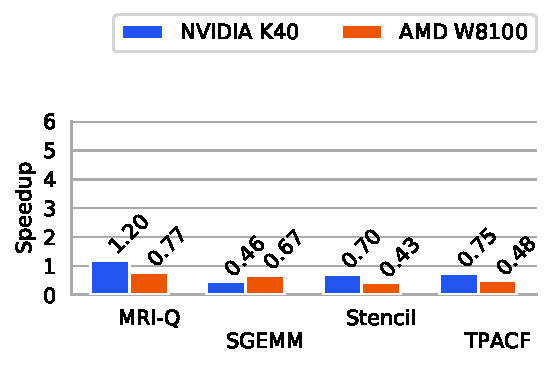
\includegraphics[scale=0.65]{experiments/parboil.pdf}
  \caption{Relative speedup compared to reference implementations for Parboil.}
  \label{fig:parboil-speedup}
\end{figure*}

The Parboil benchmark suite is smaller than Rodinia, containing $11$
benchmarks, but the implementations are generally of higher quality.
Furthermore, Parboil comes with excellent built-in support for
instrumentation and validation of results.  The Parboil benchmarks
tend to be more difficult than those found in Rodinia, so we have only
ported four of them to Futhark.  The speedups are shown on
\cref{fig:parboil-speedup}.

MRI-Q is semantically an outer \kw{map} surrounding an inner
\kw{map}-\kw{reduce} operation on an array that is invariant to the
outer \kw{map}.  The Parboil implementation is based on heavily
unrolling the inner loop, while the Futhark compiler performs
one-dimensional tiling in local memory
(\cref{sec:one-dimensional-tiling}).  This appears to be the superior
strategy on the NVIDIA GPU, but not the AMD GPU.

SGEMM is an implementation of a common matrix primitive that computes
\[
  C \leftarrow \alpha \times A \times B + \beta \times C
\]
where $A,B,C$ are matrices and $\alpha,\beta$ are scalars.  The
Futhark compiler performs two-dimensional tiling
(\cref{sec:two-dimensional-tiling}) in local memory, while the Parboil
implementation performs more sophisticated \textit{register tiling}.
SGEMM is a well-studied primitive, and it is hard for a compiler to
match a hand-tuned implementation.

Stencil is a straightforward stencil code.  The Futhark implementation
suffers due to poor memory management that induces extra copies, as
with Rodinia's HotSpot.

TPACF is semantically a histogram, which Parboil implements using
clever use of local memory.  In Futhark, we implement it using a
segmented reduction, which is not as efficient.

\subsection{Two Benchmarks from FinPar}
\label{sec:finpar}

\begin{figure*}
  \centering
  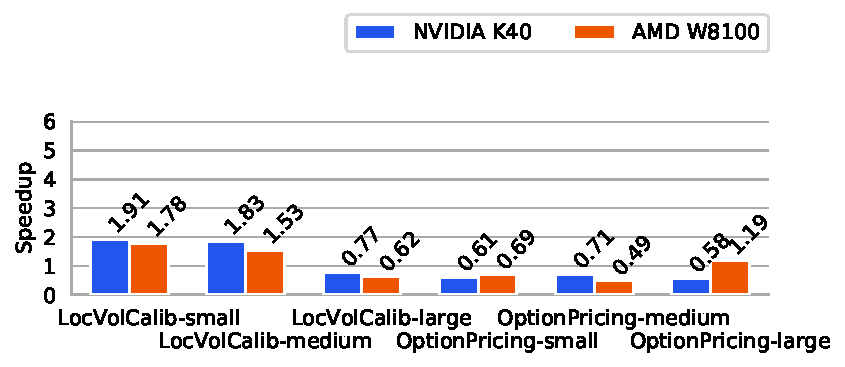
\includegraphics[scale=0.65]{experiments/finpar.pdf}
  \caption{Relative speedup compared to reference implementations for
    FinPar.  Each benchmark is applied to three different data sets.}
  \label{fig:finpar-speedup}
\end{figure*}

FinPar is a small benchmark suite translated from real-world financial
kernels.  The problems are sophisticated, with nontrivial use of
nested parallelism, and the reference implementations are well
implemented.  We have ported only two out of the three FinPar
benchmarks to Futhark, as the third one (InterestCalib) contains
(limited) irregular parallelism.  Due to the small size of FinPar, we
have evaluated each benchmark on all three available data sets.  The
speedups are shown on \cref{fig:finpar-speedup}.

OptionPricing is essentially a \kw{map}-\kw{reduce}-composition.  The
benchmark primarily measures how well the Futhark compiler
sequentialises excess parallelism inside the complex \kw{map}
function.  We see approximately equal relative performance for each of
the three data sets.

LocVolCalib from FinPar is an outer \kw{map} containing a sequential
\kw{for}-loop, which itself contains several more \kw{map}s.
Exploiting all parallelism requires the compiler to interchange the
outer \kw{map} and the sequential loop.  The slowdown on the AMD GPU
is due to transpositions, inserted to fix coalescing, being relatively
slower than on the NVIDIA GPU.

The \textit{small} and \textit{medium} datasets for LocVolCalib have
the interesting property that they do not provide enough parallelism
in the outer loops to fully saturate the GPU.  Note the absolute
runtime numbers on \cref{tab:benchmarks}, where the runtime for the
\textit{small} dataset is greater than that for the \textit{medium}
dataset, despite the latter actually requiring more work.  Two
distinct LocVolCalib implementations are provided by FinPar: one that
exploits only outer-level parallelism, and one that exploits
\textit{all} available parallelism.  The former is the right choice for
the \textit{large} dataset, and the one we compare against here, as it
is also roughly how the current Futhark compiler parallelises
LocVolCalib.  However, the FinPar implementation that fully exploits
all parallelism outperforms Futhark on the small and medium datasets.
Handling cases such as this transparently is the main motivation for
multi-versioned code (\cref{sec:multi-versioned-code}).

\subsection{Five Benchmarks from Accelerate}
\label{sec:accelerate}

\begin{figure*}
  \centering
  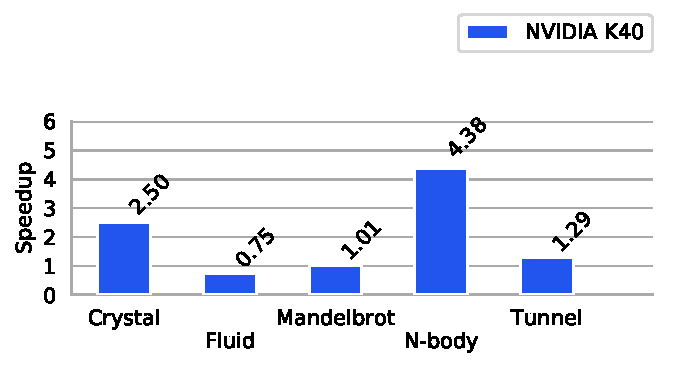
\includegraphics[scale=0.65]{experiments/accelerate.pdf}
  \caption{Relative speedup compared to reference implementations for
    Accelerate.}
  \label{fig:accelerate-speedup}
\end{figure*}

Accelerate is a mature Haskell-embedded language for data-parallel
array programming.  The benchmarks picked here are presented as
``examples'', and are not part of a benchmark suite as such.  While
they are written by the Accelerate authors themselves, and contain
built-in support for benchmarking, it is possible that performance has
been sacrificed in the interest of readability.  We use the recently
released \texttt{llvm-ptx} GPU backend, which performs significantly
better than the old \texttt{cuda} backend.  Unfortunately, this
backend is still NVIDIA-specific, so we were unable to execute
Accelerate on the AMD GPU.

The benchmarks were all straightforward to translate to Futhark, as
Accelerate does not support nested parallelism or low-level GPU
programming.  One major and interesting source of performance
differences is that Accelerate is a Just-In-Time (JIT) compiler for an
embedded language, while Futhark is a conventional Ahead-Of-Time (AOT)
compiler.  As a result, Accelerate has access to dynamic information
that can be used to perform code specialisation, but its embedded
nature limits the compilers ability to see the program as a whole.  On
the other hand, the Futhark compiler can perform more global
optimisations, but cannot inline dataset-specific constants for loop
iteration counts and similar.  The trade-offs between JIT and AOT
compilation are a fascinating and deep subject that we will not delve
further into here, but is certainly worthy of further study.  Speedups
are shown on \cref{fig:accelerate-speedup}.

Crystal is a straightforward \kw{map} containing an inner
\kw{map}-\kw{reduce} over a small array.  It is unclear why
Futhark outperforms Accelerate on this benchmark.

Fluid is a two-dimensional stencil code with complicated edge
conditions.  As with Rodinia's HotSpot, Futhark's approach to memory
management causes unnecessary copies for each of the outer sequential
loops, giving Accelerate the edge.

The Mandelbrot benchmark is a straightforward \kw{map} containing a
\kw{while} loop, with little opportunity for optimisation.

$N$-body is operationally a \kw{map} containing an inner
\kw{map}-\kw{reduce} over an array invariant to the outer array.  The
Futhark compiler performs one-dimensional tiling in local memory to
optimise access to this array.  Accelerate does not perform tiling,
which gives the edge to Futhark.

Tunnel is similar to Crystal, and contains a straightforward \kw{map}
containing an inner \kw{map}-\kw{reduce} over a small array.
Performance is similar between Futhark and Accelerate.

\subsection{Impact of Optimisations}
\label{sec:impact-of-optimisation}

Impact was measured by turning individual optimisations off and
re-running benchmarks on the NVIDIA GPU.  We report only where
the impact is non-negligible.

Fusion (\cref{chap:fusion}) has a significant impact on K-means
($\times1.42$), LavaMD ($\times4.55$), Myocyte ($\times1.66$), SRAD
($\times1.21$), Crystal ($\times10.1$), and LocVolCalib ($\times9.4$).
Without fusion, OptionPricing, N-body, MRI-Q, and SGEMM fail due to
increased storage requirements.

In the absence of in-place updates, we would have to implement K-means
as on Figure~\ref{fig:parallel-means}---the resulting program is
slower by $\times8.3$.  Likewise, LocVolCalib would have to implement
its central \lstinline{tridag} procedure via a less efficient
\lstinline{scan}-\lstinline{map} composition, causing a $\times1.7$
slowdown.  OptionPricing uses an inherently sequential Brownian Bridge
computation that is not expressible without in-place updates.

The coalescing-by-transposition transformation
(\cref{sec:automatic-coalescing}) has a significant impact on
$k$-means ($\times9.26$), Myocyte ($\times4.2$), OptionPricing
($\times 8.79$), and LocVolCalib ($\times 8.4$).
%
Loop tiling (\cref{sec:automatic-tiling}) has an impact on LavaMD
($\times 1.35$), MRI-Q ($\times1.33$), SGEMM ($\times2.3$), $N$-body
($\times 2.29$), and LUD ($\times 1.10$).

\section{Benchmarking an implementation of Breadth-First-Search}
\label{sec:bfs-benchmarking}

The Rodinia benchmark suite contains a benchmark, BFS, that
implements Breadth-First-Search.  This problem is highly irregular,
and its performance is very dataset-sensitive.  As a result, we have
excluded it from the presentation of the general benchmark results,
and instead dedicated this section to discuss the issues.  The
following serves as an example of benchmarks where measuring
performance is not quite straightforward, and incidentally as an
example of how to implement irregular problems in Futhark.

Figure~\ref{fig:bfs-imperative} shows an excerpt of Rodinia's
imperative-but-parallel implementation of the breadth-first search
algorithm, which traverses the graph and records in the
\lstinline{cost} array the breadth level of each graph node.
%
The code excerpt processes in parallel all the nodes, indexed by \lstinline{src_id},
on the current breadth level (i.e., the ones with the \lstinline{mask[src_id]} set).
%
For each such node, the breadth level of all its unvisited neighbours
(i.e., \lstinline{!visited[id]}) are updated to \lstinline{cost[src_id]+1} in the
sequential (inner) loop at line \ref{line:seqcostupd}.
%
The problem with this code is that the update of \lstinline{cost}
potentially introduces data races in the case when two nodes on the
same level are connected to a common (unvisited) node.  What makes it
still safe is the property that the output dependences are idempotent
(i.e., the updated value is the same across different outermost
iterations).

Figure~\ref{fig:bfs-fun-pad} shows a simple, albeit work-inefficient,
translation to Futhark of the discussed imperative code, which uses
padding to satisfy array regularity. First, the indices of the active
nodes (i.e., the ones on the current breadth level) are identified by
the \lstinline{filter} operation on line \ref{line:futfilter}.  This
contributes significantly to final performance.  Second, the maximal
number of edges of these nodes, denoted by \lstinline{e_max}, is
computed via a \lstinline{map-reduce} composition on lines
\ref{line:emaxstart}--\ref{line:emaxend}.  Third, the \lstinline{map}
nest computes two two-dimensional arrays of innermost size equal to
\lstinline{e_max}, in which the first one corresponds to the indices
of the unvisited neighbours, and the second one to their breadth level
(\lstinline{costs}).  The indices that are outside the edge degree of
a node are marked with out-of-bounds indices (\lstinline{-1}), and
similarly for the nodes that were already visited.
%
Fourth, the index-value arrays are flattened (at lines
\ref{line:futflatstart}-\ref{line:futflatend}) and the
\lstinline{scatter} bulk operator is used to update the
\lstinline{cost} and \lstinline{updating_mask} arrays at lines
\ref{line:futupdatestart}--\ref{line:futupdateend}.

Table~\ref{fig:bfs-speedup} shows the running time of Futhark and
Rodinia implementations on four datasets. The Rodinia implementation
exploits only the parallelism of the outer loop, and it wins on the
datasets in which the graph is large enough to fully utilise the
hardware, while Futhark exploits both levels of parallelism and wins
on smaller graphs with large edge degree.  Interestingly, this is not
simply a question of how much to parallelise, but a fundamental
algorithmic design decision.  The unsolved challenge is a
representation and technique that can fuse the Futhark code in
\cref{fig:bfs-fun-pad} into something resulting the one-level-parallel
C code in \cref{fig:bfs-imperative}, and furthermore generate both
versions of the code.

\begin{figure}[ht]
\begin{lstlisting}[xleftmargin=0pt,language=C,numbers=left,escapechar=|]
// n is the number of graph nodes
for (int src_id = 0; src_id < n; src_id++ ) { // parallel
    if (mask[src_id] == true) {
        mask[src_id] = false;
        for (int i = nodes[src_id].starting; // sequential
             i < (nodes[src_id].num_edges
                  +nodes[src_id].starting);
             i++) {
            int dst_id = edges_dest[i];
            if(!visited[dst_id]) {
                cost[dst_id] = cost[src_id] + 1; |\label{line:seqcostupd}|
                updating_mask[dst_id] = true;
            }
        }
   }
}
\end{lstlisting}
  \caption{Imperative code for breadth-first search.}
  \label{fig:bfs-imperative}
\end{figure}

\begin{figure}[ht]
\small
\begin{lstlisting}[xleftmargin=0pt,language=futhark,numbers=left,escapechar=|]
let step [n][e] (cost: [n]i32)
                (nodes_starting: [n]i32)
                (nodes_num_edges: [n]i32)
                (edges_dest: [e]i32)
                (visited: [n]bool)
                (mask: [n]bool)
    : ([n]i32, [n]bool, []i32) =
  let active_indices = filter (\i -> mask[i]) (iota n)|\label{line:futfilter}|
  let n_indices = length active_indices
  let e_max = |\label{line:emaxstart}|
    reduce i32.max 0
    (map (\i -> nodes_n_edges[i]) active_indices)|\label{line:emaxend}|
  let (node_ids_2d, costs_2d) =
    map (\src_id: ([e_max]i32, [e_max]i32)  ->
          let s_index = nodes_starting [src_id]
          let n_edges = nodes_num_edges[src_id]
          let edge_indices = map (+s_index) (iota e_max)
          let node_ids =
            map (\i ->
                  if i < s_index + n_edges
                  then let dst_id = edges_dest[i]
                       in  if !visited[dst_id]
                           then dst_id else -1
                  else -1)
                edge_indices
          let costs = replicate e_max (cost[src_id] + 1)
          in (node_ids, costs))
         active_indices
  let node_ids = reshape flat_len node_ids_2d |\label{line:futflatstart}|
  let costs = reshape flat_len costs_2d |\label{line:futflatend}|
  let flat_len = e_max * n_indices
  let mask' = |\label{line:futupdatestart}|
    scatter mask active_indices (replicate n_indices false)
  let cost' =
    scatter cost node_ids costs
  let updating_mask' =
    scatter updating_mask node_ids (replicate flat_len true) |\label{line:futupdateend}|
  in (mask', cost', updating_mask')
\end{lstlisting}
  \caption{Work-inefficient Futhark code for breadth-first search.}
  \label{fig:bfs-fun-pad}
\end{figure}

Finally, we remark that the presented Futhark code is work-inefficient
due to the ``padding'' of the edge-degree of a node, but the
\lstinline{scatter} construct also enables a work-efficient
implementation (not shown), which corresponds to full flattening. In
our tests, this is slower than the padded one due to the overhead of
multiple scans.
%

\begin{table*}
  \centering
  \begin{tabular}{llrr}
    \textbf{Dataset} & \textbf{Version} & \textbf{Runtime} & \textbf{Speedup} \\

    \multirow{2}{*}{2000 nodes, 1000 edges each} & Futhark & 4.0ms & \multirow{2}{*}{$\times1.9$} \\\cline{2-3}
                     & Rodinia & 7.6ms \\\hline

    \multirow{2}{*}{1000 nodes, 10--1000 edges each} & Futhark & 1.7ms & \multirow{2}{*}{$\times3.7$} \\\cline{2-3}
                     & Rodinia & 6.3ms \\\hline

    \multirow{2}{*}{100,000 nodes, 6 edges each} & Futhark & 6.7ms & \multirow{2}{*}{$\times0.25$} \\\cline{2-3}
                     & Rodinia & 1.7ms \\\hline

    \multirow{2}{*}{100,000 nodes, 10--500 edges each} & Futhark & 153.1ms & \multirow{2}{*}{$\times0.43$} \\\cline{2-3}
                     & Rodinia & 66.5ms \\\hline

  \end{tabular}
  \caption{Performance of Rodinia and Futhark breadth-first search
    implementations on various datasets. Executed on an NVIDIA GTX 780
    Ti with random graphs (uniform distribution).  Reported runtime is
    average over $10$ runs.}
  \label{fig:bfs-speedup}
\end{table*}

%%% Local Variables:
%%% mode: latex
%%% TeX-master: "thesis"
%%% End:
